\documentclass[10pt]{exam}
\usepackage[hon]{template-for-exam}
\usepackage{tikz,multicol}
\usetikzlibrary{shadings,shadows}


\title{Angular Quantities}
\author{Rohrbach}
\date{\today}

\begin{document}
\maketitle

\section*{Measuring Angles}
\begin{tikzpicture}
  \draw[dotted] (0,3) -- (0,-3);
  \draw[dotted] (3,0) -- (-3,0);
  \draw[thin] circle (2);
  \path (2,0) coordinate (b);
  \draw[ultra thick, red] (b) arc (0:57.29:2)
    coordinate (e);
  \draw[dashed,red] (0,0) -- (e);
  \draw[dashed,red] (0,0) -- (b);
\end{tikzpicture}
%
\hfill
%
\begin{tikzpicture}[scale=0.7]
  \draw[dotted] (0,3) -- (0,-3);
  \draw[dotted] (3,0) -- (-3,0);
  \draw[thin] circle (2);
  \path (2,0) coordinate (b);
  \draw[ultra thick, blue] (b) arc (0:120:2)
    coordinate (e);
  \draw[dashed,blue] (0,0) -- (e);
  \draw[dashed,blue] (0,0) -- (b);
\end{tikzpicture}
\vs

\section*{Conversions}
\vs



\section*{Angular Kinematic Quantities}

\renewcommand{\arraystretch}{2}

\begin{tabular}{p{9em}ccp{6.5em}}
  Concept & Linear/Translational Quantity & Angular/Rotational Quantity & \hfill ``Bridge'' \\ \hline\hline
  position \\[2em]\hline
  displacement \\[1em] & units: & units:  \\\hline
  velocity \\[1em] & units: & units:  \\\hline
  acceleration \\[1em] & units: & units: \\\hline
\end{tabular}


\pagebreak


\section*{Practice}

\begin{questions}
  
\question 
  When you look at the Sun from the surface of the Earth, it subtends an angle of about 0.5$^\circ$ in the sky.  The Earth is 150 million km away from the Sun.  (a) Convert your angle to radians.  (b) Estimate the diameter of the Sun.

  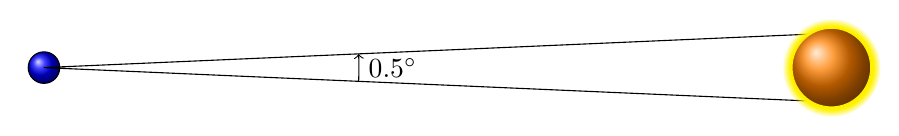
\begin{tikzpicture}
    \draw[shading=ball] (0,0) circle (0.2);
    \draw (2.5:10) -- (0,0) -- (-2.5:10);
    \draw[->] (-2.5:4) arc (-2.5:2.5:4) 
      node[midway,anchor=west] {$0.5^\circ$};
    \fill[
      shading=ball, 
      ball color=orange,
      circular glow={fill=yellow}, 
      draw=yellow
    ] 
    (10,0) circle (.5);
  \end{tikzpicture}

  \vs

\question
  A bicycle has wheels of diameter 68 cm. If the bicycle travels 92 km, how many rotations do the wheels make?
  \vs


\question
  A wheel of radius 1.3 meters is accelerating at a rate of 12 rad/s$^2$. At the moment that the wheel is rotating at 3.2 rad/s,
  %
  \begin{parts}
    \part what is the magnitude of \emph{tangential} acceleration at a point on the outside of the wheel?
    \part what is the magnitude of \emph{radial} (centripetal) acceleration at a point on the outside of the wheel?
    \part what is the magnitude of the \emph{total} acceleration at a point on the outside of the wheel?
  \end{parts}
  \vs

\end{questions}


\end{document}